\section{Filtertype: Aktive og Passive}
\label{Filtertype}
%\begin{itemize}
%  \item Aktivt eller passivt filter inklusiv komponenter
%  \item Fordele og ulemper
%  \item Illustration 
%  \item Bestem at det er et aktivt filter vi skal bruge
%\end{itemize}
Filtre kan være enten passive eller aktive, hver med sine egenskaber. Hvilken filtertype man vælger, afhænger af hvilke egenskaber man ønsker, såvel som krav til pris og fysisk størrelse. I følgende sektion, tages udgangspunkt i lavpasfiltre, omend de generelle egenskaber også er gældende for høj- og båndpasfiltre.\\
Passive filtre, som set på \autoref{fig:LowPassPassive} har den fordel at de kan operere uden tilført strøm, som navnet angiver. De benytter kun passive komponenter som modstande, kondensatorer og spoler og virker bedst ved frekvenser mellem 100Hz og 300MHz \parencite{BOOK:PracticalElectronicsforInventors}. Dets lavere frekvensområde, dets større kapacitans og induktans, hvilket kræver fysisk større komponenter, deraf den nedre grænse. Ved høje frekvenser vil komponenterne interferere med hinanden, deraf den øvre grænse.
%
\begin{figure}[H]
	\centering
	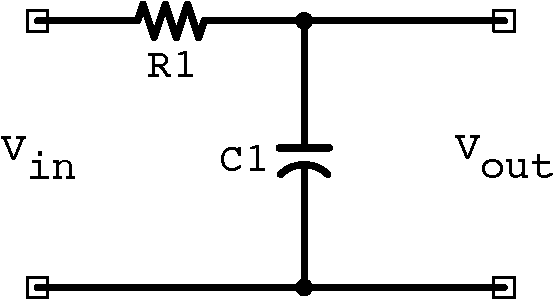
\includegraphics[resolution=300,scale=\diagramSize]{Introduktion/LowPassPassive}
	\caption{Et simpelt passivt filter}
	\label{fig:LowPassPassive}
\end{figure}
\noindent
%
Aktive filtre, som set på \autoref{fig:LowPassActive}, kræver tilført strøm, og benytter en operationsforstærker (OpAmp), sammen med modstande og kondensatorer. De kan håndtere meget lave frekvenser og kan øge spændingen på output, hvis ønsket. De er ofte nemmere at konstruere end passive filtre, og kan laves uden brug for store komponenter. De virker bedst ved frekvenser under 100kHz, som konsekvens af operationsforstærkerens båndbredde og slew-rate \parencite{BOOK:PracticalElectronicsforInventors} \fxnote{Hvad hedder slew rate på dansk?}.
%
\begin{figure}[H]
	\centering
	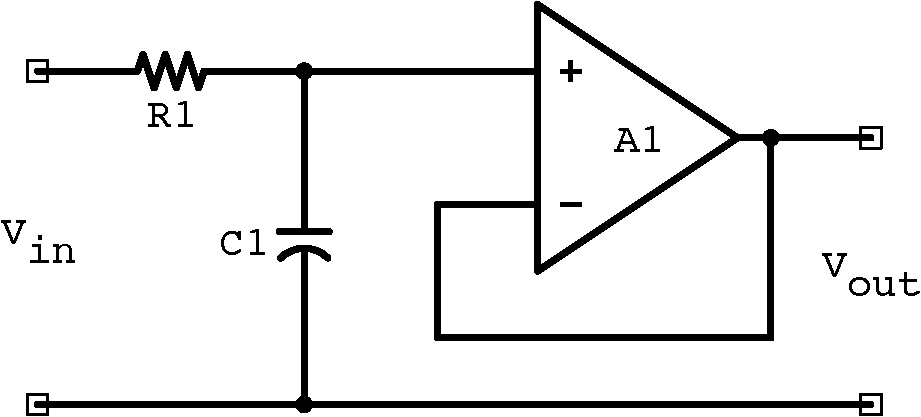
\includegraphics[resolution=300,scale=\diagramSize]{Figure/Introduktion/ActiveLowPass.pdf}
	\caption{Et simpelt aktivt filter, uden gain}
	\label{fig:LowPassActive}
\end{figure}
\noindent
%
Eftersom at mennekser kan høre lyde mellem ca. 20Hz og 20kHz \fxsource, er et aktivt filter at foretrække, da det er bedre egnet end passive filtre, i dette frekvensområde. Af samme årsag vil resten af denne rapport beskæftige sig med disse.
%
%
%
\section{Lavpasfiltre}
\label{Lavpasfiltre}
\begin{itemize}
  \item Knækfrekvenser
  \item Overførringsfunktionen
  \item Hældning 
  \item Formål 
  \item Illustrationer
  \item Formler
  \item Bode-plots?
  \item Brug afsnittet omkring hældningen i det lavfrekventeområde
\end{itemize}
Et lavpasfilter er et filter der, som navnet antyder, lader lave frekvenser passere igennem, men blokerer for høje. På \autoref{fig:LowPassActive} ses et aktivt lavpasfilter. At det er aktivt, betyder blot at der benyttes en operationsforstærker i sammenhæng med filtret.\\
Et lavpasfilter virker ved at kondensatoren, ved høje frekvenser, sænker sin impedans og således lader højre frekvenser gå til jord i stedet for at passere. Modstanden har stor impedans ved høje frekvenser, men lader lave frekvenser passere.\\
I opkoblingen fra \autoref{fig:LowPassActive} er der ingen forstærkning af inputsignalet, eftersom tilbagekoblingen går urørt fra $V_{out+}$ til operationsforstærkerens $V_{in-}$. En sådan tilbagekobling kan have fordele, selvom der ikke sker nogen forstærkning. Operationsforstærkerens høje inputimpedans forhindrer overdrevet belastning af filterets output og dens lave outputimpedans sørger for at filtrets afskæringsfrekvens ikke påvirkes af eventuelle ændringer af den efterfølgende impedans. Selvom filteret fra \autoref{fig:LowPassActive} ikke giver nogen spændingsforstærkelse over 1, giver det en meget høj effekt, grundet at inputimpedansen er langt højere end outputimpedansen. Med andre ord giver det god stabilitet til filteret. Et kredsløb med forstærkning, kan ses på \autoref{fig:LowPassActiveGain.pdfGain}.
%
\begin{figure}[H]
	\centering
	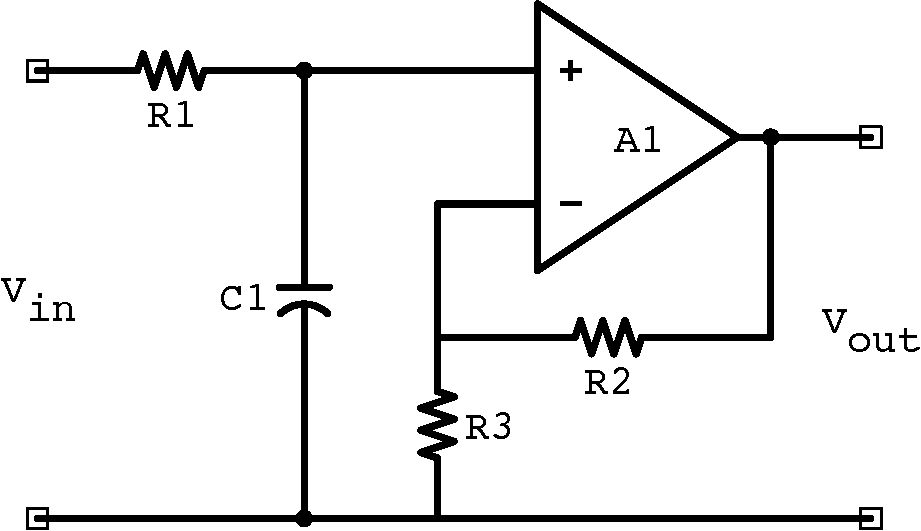
\includegraphics[resolution=300,scale=\diagramSize]{Figure/Introduktion/ActiveLowPassGain.pdf}
	\caption{Aktivt lavpasfilter med forstærkning}
	\label{fig:LowPassActiveGain}
\end{figure}
\noindent
\fxnote{Opdatér figur til ny stil}
%
%
%Forholdet mellem modstandene R1 og R2 dikterer $DC$-forstærkningen, og følger, for en ikke-inverterende operationsforstærker, formlen:
%%
%\begin{equation} \label{eq:LowPassDCGain}
%	DC_{gain}=\left(1+\frac{R_2}{R_1}\right)
%\end{equation}
%%
%Sammenholdt med filteret, følger den frekvensafhængige forstærkning af et lavpasfilter således formlen:
%%
%\begin{equation} \label{LowPassFqVGain}
%  V_{gain}=\frac{V_{out}}{V_{in}}=\frac{A_F}{\sqrt{1+\left(\frac{f}{f_c}\right)^2}}
%\end{equation}
%Hvor:\\
%$A_F$ = Forstærkningsfaktoren for operationsforstærkeren, $DC_{gain}$\\
%$f$ = Frekvensen af inputsignalet, i Hz\\
%$f_c$ = Afskæringsfrekvensen for filteret, i Hz\\
%Filteret har konstant forstærkning, $A_F$, fra 0Hz til lidt før afsksæringsfrekvensen $f_c$, hvorefter amplituden falder med en konstant rate på 20dB pr. dekade. Forløbet kan ses på \autoref{fig:FrequencyResponseCurve}.
%%
%\begin{figure}[H]
%	\centering
%	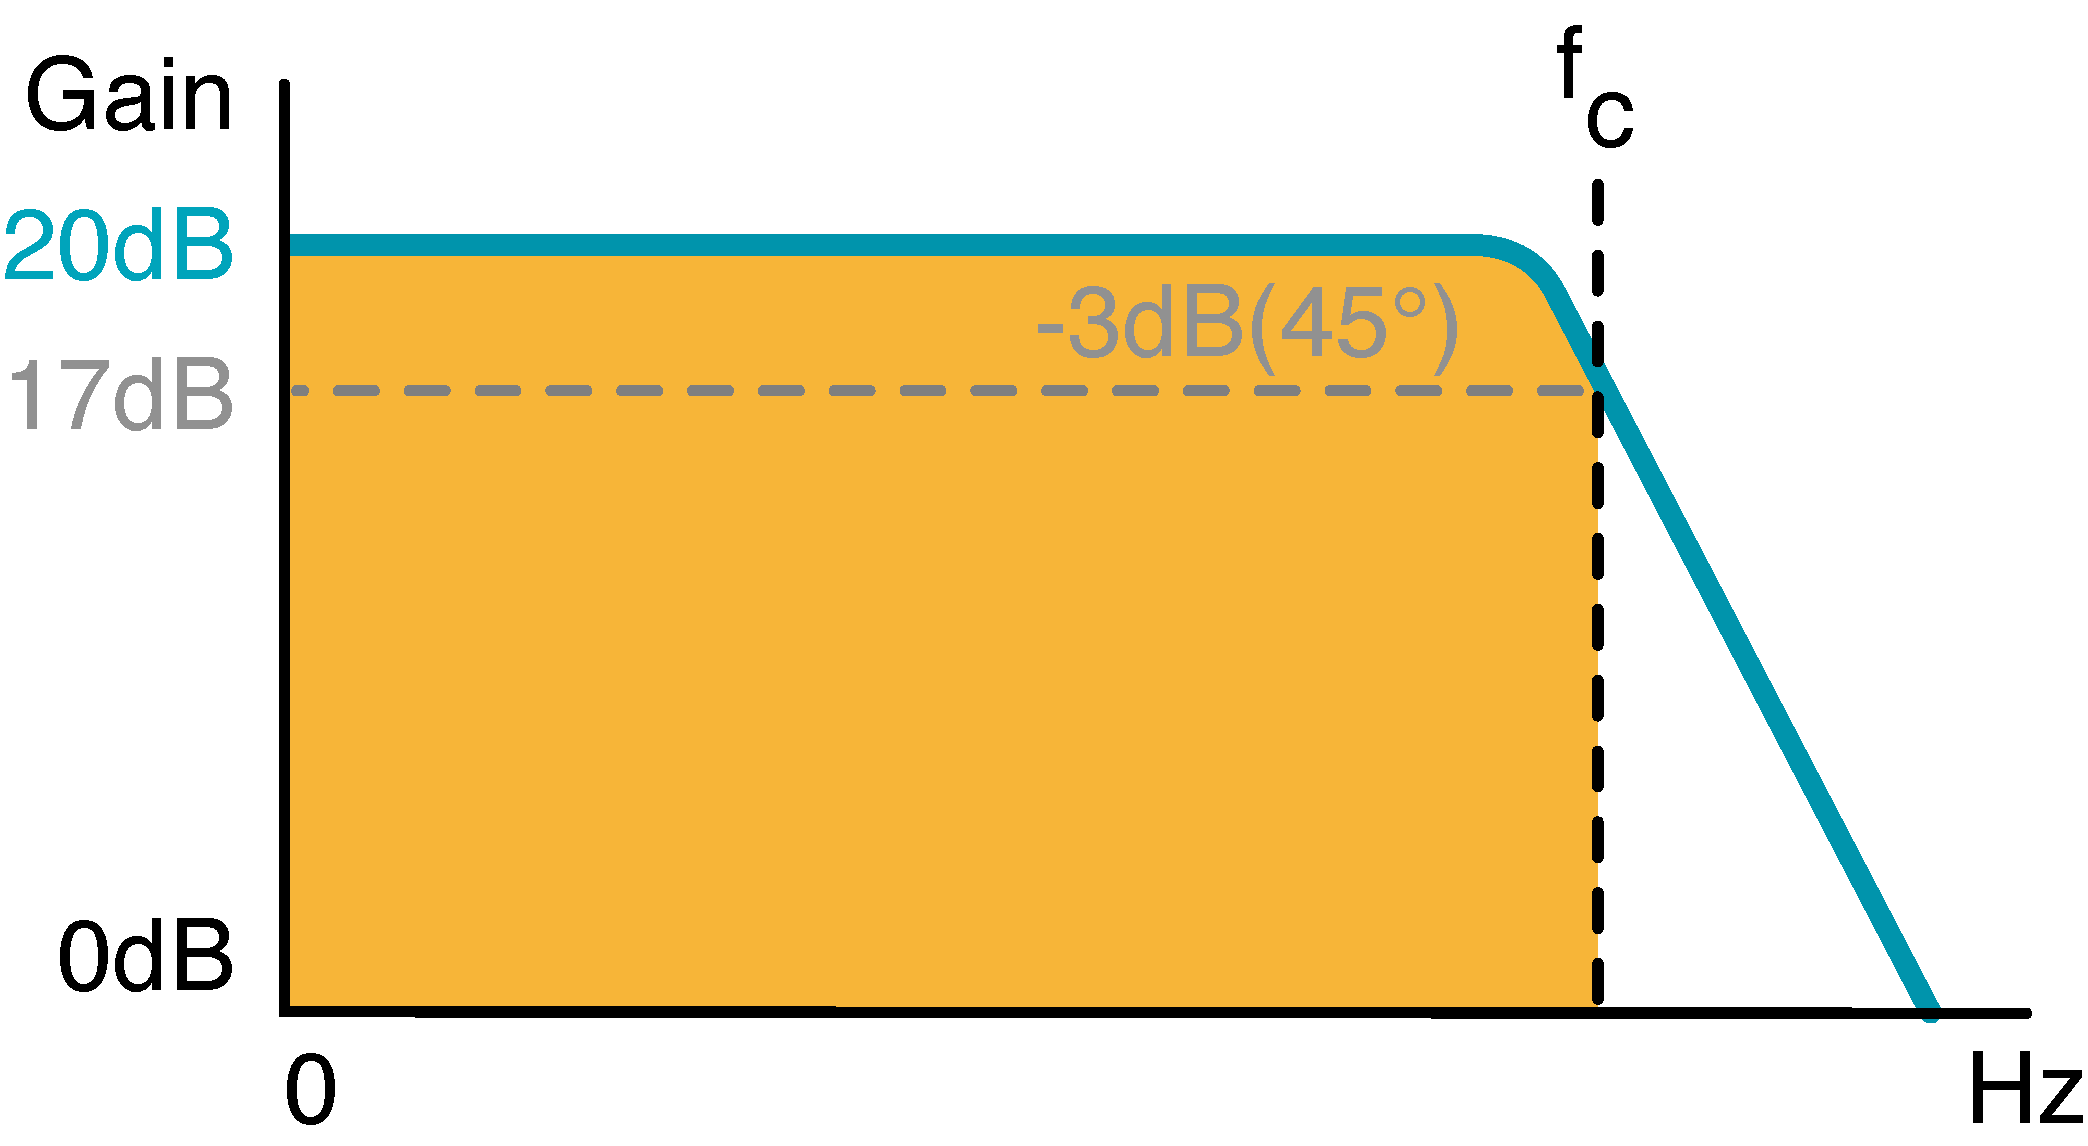
\includegraphics[resolution=300,width=\textwidth/2]{Introduktion/FrequencyResponseCurve}
%	\caption{Frekvensresponskurve for et lavpasfilter. Den orange del, er det frekvensområde som medtages i}
%	\label{fig:FrequencyResponseCurve}
%\end{figure}
%\noindent
%
%
%
\subsection{Fraktalordensfilter}
\label{Fraktalordensfilter}
%
\begin{itemize}
  \item Knækfrekvenser (fåes fra behandling af ISO)
  \item Hældning (fåes fra hældning i det lavfrekventeområde)
  \item Pinknoise filter? (hældning på 10dB/dec)
  \item Bode-plots
  \item Illustrationer
  \item Formler
  \item Hvorfor vi bruger fraktalordensfilter
\end{itemize}
\noindent
%
For at finde ud af hvilken orden vores filter skal være bruges formlen 
\begin{equation}
	a=20*log(10^x)
\end{equation}

%
\subsubsection{Hældning i det lavfrekventeområde}
\label{HaeldningIDetLavfrekventeområde}
%
\begin{itemize}
	\item Bruges til at bestemme hældningen på lavpas-filtrene.
	\item Vi vil gerne lave et filter, som kan sættes efter hinanden for at få en større hældning så derfor runder vi op til hele 5'ere, da den afrundning vil være uhørbar
\end{itemize}

I \autoref{tab:ISO226Difference630Hz} forefindes det nye datasæt i frekvensområdet fra 20Hz til 630Hz, hvor de resterende datapunkter forefindes i \autoref{app:ISO226Difference}. 
%
\begin{table}[H]
\centering
\resizebox{\textwidth}{!}{%
\begin{tabular}{|r|r|r|r|r|r|r|r|r|}
\hline
\multicolumn{1}{|l|}{Frekvens{[}Hz{]}} & \multicolumn{1}{l|}{20phon} & \multicolumn{1}{l|}{30phon} & \multicolumn{1}{l|}{40phon} & \multicolumn{1}{l|}{50phon} & \multicolumn{1}{l|}{60phon} & \multicolumn{1}{l|}{70phon} & \multicolumn{1}{l|}{80 phon} & \multicolumn{1}{l|}{90phon} \\ \hline
20 & 30.6 & 25.8 & 20.9 & 15.7 & 10.5 & 5.3 & 0 & -5.3 \\ \hline
25 & 28.5 & 24.3 & 19.7 & 14.9 & 10 & 5 & 0 & -5 \\ \hline
31.5 & 26.4 & 22.8 & 18.6 & 14.1 & 9.5 & 4.8 & 0 & -4.7 \\ \hline
40 & 24.6 & 21.2 & 17.3 & 13.2 & 8.9 & 4.5 & 0 & -4.4 \\ \hline
50 & 22.3 & 19.6 & 16.1 & 12.3 & 8.3 & 4.2 & 0 & -4.2 \\ \hline
63 & 20.2 & 17.8 & 14.7 & 11.2 & 7.5 & 3.8 & 0 & -3.9 \\ \hline
80 & 18 & 16 & 13.3 & 10.2 & 6.9 & 3.4 & 0 & -3.5 \\ \hline
100 & 15.9 & 14.3 & 11.9 & 9.1 & 6.2 & 3.1 & 0 & -3.2 \\ \hline
125 & 13.8 & 12.5 & 10.5 & 8.1 & 5.5 & 2.8 & 0 & -2.8 \\ \hline
160 & 11.6 & 10.6 & 8.9 & 6.9 & 4.7 & 2.4 & 0 & -2.4 \\ \hline
200 & 9.6 & 8.9 & 7.5 & 5.8 & 4 & 2 & 0 & -2 \\ \hline
250 & 7.7 & 7.2 & 6.1 & 4.7 & 3.2 & 1.6 & 0 & -1.7 \\ \hline
315 & 5.8 & 5.5 & 4.7 & 3.6 & 2.5 & 1.3 & 0 & -1.3 \\ \hline
400 & 4 & 3.8 & 3.3 & 2.6 & 1.8 & 0.9 & 0 & -0.9 \\ \hline
500 & 2.5 & 2.5 & 2.2 & 1.7 & 1.2 & 0.6 & 0 & -0.7 \\ \hline
630 & 1.3 & 1.3 & 1.1 & 0.9 & 0.6 & 0.3 & 0 & -0.4 \\ \hline
\end{tabular}%
}
\caption{Det nye datasæt, som består af differencerne mellem referencen og de specifikke phon-kurver, samt lydtryksniveauerne målt ved hver frekvens. Datasættet fokuserer kun på frekvensområdet 20Hz til 630Hz.}
\label{tab:ISO226Difference630Hz}
\end{table}
%


\begin{table}[H]
\centering
\resizebox{\textwidth}{!}{%
\begin{tabular}{|r|r|r|r|r|r|r|r|r|}
\hline
\multicolumn{1}{|l|}{Frekvens{[}Hz{]}} & \multicolumn{1}{l|}{20phon} & \multicolumn{1}{l|}{30phon} & \multicolumn{1}{l|}{40phon} & \multicolumn{1}{l|}{50phon} & \multicolumn{1}{l|}{60phon} & \multicolumn{1}{l|}{70phon} & \multicolumn{1}{l|}{80 phon} & \multicolumn{1}{l|}{90phon} \\ \hline
20-630 & 29.3 & 24.5 & 19.8 & 14.8 & 9.9 & 5 & 0 & 0 \\ \hline
\end{tabular}%
}
\caption{Hældningen mellem 20Hz og 630Hz for hver phon-kurve, udregnet ved differencen derimellem.}
\label{tab:HaeldningFra20til630}
\end{table}
\noindent
%
Brugt til at finde stepsize på vores filter, så når der er en ændring i volumen på 5dB skal vi skifte filter. 

\begin{table}[H]
\centering
\resizebox{\textwidth}{!}{%
\begin{tabular}{|r|r|r|r|r|r|r|r|r|}
\hline
\multicolumn{1}{|l|}{Frekvens{[}Hz{]}} & \multicolumn{1}{l|}{20phon} & \multicolumn{1}{l|}{30phon} & \multicolumn{1}{l|}{40phon} & \multicolumn{1}{l|}{50phon} & \multicolumn{1}{l|}{60phon} & \multicolumn{1}{l|}{70phon} & \multicolumn{1}{l|}{80 phon} & \multicolumn{1}{l|}{90phon} \\ \hline
20-200 & 21 & 16.9 & 13.4 & 9.9 & 6.5 & 3.3 & 0 & -3.3 \\ \hline
200-630 & 8.3 & 7.6 & 6.4 &4.9 & 3.4 & 1.7 & 0 & -1.6\\ \hline
200-2000 & 12 & 10.7 & 8.9 & 6.8 & 4.6 & 2.3 & 0 & -2.3\\ \hline
\end{tabular}%
}
\caption{Hældningen per dekade, udregnet ved differencen derimellem.}
\label{tab:HaeldningFra20til630}
\end{table}
\noindent
%
Bruges til at finde den hældning vores filter skal have. De tal der står der skal halveres fordi de er regnet med en stepsize på 10dB, så ved 70phon (mellem 20 og 200) skal 3.3 dB være 1.7 dB (1.65)?. Hældningen ville være 3.3 dB per 2 dekader. 

\section{Operationsforstærker}
\label{OpAmp}
%
\begin{itemize}
  \item Ideelle og reelle operationsforstærkere
  \item Inverterende og ikke-inverterende 
  \item Illustrationer
  \item Formler
  \item Tilbagekobling - hvorfor er det godt? 
  \item Beta-værdier og udregninger 
\end{itemize}

\section{Dimensionering af fraktalordens lavpasfilter}
\label{DimensioneringAfFraktalordensLavpasfilter}
%
\begin{itemize}
  \item Signalet vej igennem vores filter
  \item Komponent valg og værdier (modstande, kondensatorer, operationsforstærker mm.) 
  \item Beregninger af komponent værdier
  \item Illustrationer og simulationer
\end{itemize}




